\chapter{Technical Background}

Over the course of the past decade, elliptic curve cryptography (henceforth referred to as ECC) has proven itself a mainstay in the wide world of applied Cryptology. While Isogeny based cryptography does build itself up from the same underlying mathematical concepts as ECC, it simultaneously draws from a slightly more complicated space of niche algebraic notions. Much of this chapter will be dedicated to illuminating these notions in a manner that should be digestable for those without serious background in algebraic geometry, or abstract algebra in general.

This chapter will cover the following preliminary topics: isogenies and their relevant properties, Supersingular Isogeny Diffie-Hellman and its related procotols, the Fiat-Shamir construction and its quantum-safe adaptation, and finally the current landscape of isogeny based signature schemes.

Our discussion of Isogenies will begin with some basic coverage of the underlying algebra. We will provide the material necessary for the remaining sections as we build up in the level of abstraction; working our way through finite fields, elliptic curves, and finally isogenies and their properties.

Once we have presented the necessary algebra, we will illustrate the specifics of the supersingular isogeny Diffie-Hellman key-exchange protocol. We will spend most of this time dedicated to a modular deconstruction of the protocol, laying bare the underlying isogeny-level procedures and algorithms that will be necessary for understanding the protocols to come in detail. Another task of this section will be to introduce the SIDH C library released by Microsoft Research, on top of which the core contributions of this thesis are implemented. This subsection will end with a thorough briefing and analysis of the closely related zero-knowledge proof of identity isogeny protocol proposed in the original JDP paper, as it is necessary for understanding the isogeny based signature scheme presented by Yoo et. Al.\\

\section{Algebraic Geometry \& Isogenies}

Let us begin with some group $G$. $G$ is said to be an $abelian$ group if, in addition to the four traditional group axioms, $G$ satisfies the condition of commutitiviy. More formally: for some group $G$ with group operation $\cdot$, we say $G$ is an abelian group iff $x \cdot y = y \cdot x$ $\forall x, y \in G$.\\

A \emph{morphism} is the somewhat general notion of a structure-preserving map. Morphisms can be thought of as functions from some mathematical structure ($A$) to another ($B$). More specifically, in the domain of algebraic geometry, we will be dealing with the notion of a \emph{group homomorphism}, defined as follows:
\begin{definition}[Group Homomorphism]
\label{defn:homomorphism}
For two groups $G$ and $H$ with group operations $*$ and $\cdot$ respectively, a \emph{group homomorphism} is a mapping $h: G \rightarrow H$ such that $\forall u, v \in G$ the following holds:
$$h(u * v) = h(u) \cdot h(v)$$
\end{definition}
From this simple definition, two more properties of homomorphisms are easily deducible. Namely, for some homomorphism $h: G \rightarrow H$, the following properties hold:
\begin{itemize}
\item $h$ maps the identity element of $G$ onto the identity element of $H$
\item $h(u^{-1}) = h(u)^{-1}, \forall u \in G$
\end{itemize}
Furthermore, an \emph{endomorphism} is a special type of morphism in which the domain and the codomain are the same mathematical object.

\subsection{Elliptic Curves}

geometry stuff:
An elliptic curve is an algebraic curve defineable by an equation of the form $y^2 = x^3 + ax + b$.
The point at infinity.

algebra stuff:
elliptic curves over finite fields are abelian varieties. 
group to abelian group to abelian variety to morphism/homomorphism to isogenies are homomorphisms over abelian varieties.

\begin{figure}[htb]
\centering
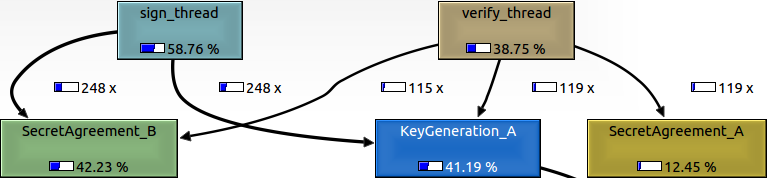
\includegraphics[scale=0.3]{signandverifycall.png} % e.g. insert ./image for image.png in the working directory, adjust scale as necessary
\caption{Temporary. To be replaced with illustration of EC group operation.}
\label{fig:label} % insert suitable label, this is used to refer to a fig from within the text as shown above
\end{figure}

blah blah the points on an elliptic curve defined over some finite field form an abelian variety

\subsection{Supersingular Curves}

An elliptic curve can be either \emph{ordinary} or \emph{supersingular}. There are several equivalent ways to define supersingular curves (and thus the distinction between them and ordinary curves,)

For the remainder of this paper, unless otherwise noted, all elliptic curves in discussion will be of the supersingular variety.

\subsection{Isogenies \& Their Properties}

An isogeny is a certain sort of \emph{function} or \emph{map} which is defined in relation to the earlier discussed concept of a homomorphism[link]. The formal definition is as follows:\\
\begin{definition}[Isogeny]
\label{defn:isogeny}
Let $G$ and $H$ be abelian varieties[ref]. An isogeny is a homomorphism[ref] $h: G \rightarrow H$ possessing a finite kernel.
\end{definition}

\section{Supersingular Isogeny Diffie-Hellman}

This section will aim to accomplish two things. First, we will briefly explain the isogeny-level procedures of the SIDH protocol. Second, we will illuminate how these procedures map onto Microsoft's C library for SIDH. In this regard, this section can be considered an attempt to meld two domains of SIDH functions \& procedures, in hopes of easing the process of navigation from the SIDH scheme to Microsoft's C implementation, and vice versa.

SIDH protocols, as the name suggests, work over supersingular curves of smooth order. Let $\mathbb{F}_q = \mathbb{F}_{p^2}$ be the finite field over which our curve is defined. $p$ is a prime defined as follows:
$$
p = \ell_{A}^{e_A}\ell_{B}^{e_B} \cdot f \pm 1
$$
Wherein $\ell_{A}$ and $\ell_{B}$ are small primes (typically 2 \& 3, respectively) and $f$ is a cofactor ensuring the primality of $p$.

\subsection{Modular Breakdown}

	Before drawing parallels between the SIDH protocol and its C implementation, we will first offer a brief digest of the libraries unit organization.\\

\begin{center}
Header files:\\
	\begin{tabular}{@{}ll@{}}
		File & Description of contents\\
		\toprule
		SIDH.h & \\
		\midrule
		SIDH\_internal.h & \\
		\midrule
		SIDH\_api.h & \\
		\midrule
		keccak.h & \\
		\bottomrule
	\end{tabular}\\
	
Source files:\\
	\begin{tabular}{@{}ll@{}}
		File & Description of contents\\
		\toprule
		SIDH.c & \\
		\midrule
		kex.c & \\
		\midrule
		ec\_isogeny.c & \\
		\midrule
		fpx.c & \\
		\midrule
		keccak.c & \\
		\midrule
		sha256.c & \\
		\bottomrule
	\end{tabular}\\
	
Test files:\\
	\begin{tabular}{@{}ll@{}}
		File & Description of contents\\
		\toprule
		kex\_tests.c & Correctness \& performance tests for key exchange\\
		\midrule
		arith\_tests.c & Correctness \& performance testing of field arithmetic\\
		\bottomrule
	\end{tabular}
\end{center}

\textbf{Ephemeral Key Generation -- Alice}:

	\parbox[t]{.35\linewidth}{
	\centering
	Key generation for Alice
	\begin{tabular}{@{}ll@{}}
		\toprule
		Location & Efficient Algo's Appendix A \\
		\midrule
		Input & $x_{P_{B}}, x_{P_{A}}, y_{P_{A}}$,\\
		& $SK_{Alice}$ = $m_{A} \cdot l_{A}$\\
		\midrule
		Output & $PK_{Alice}$ = $[x_{\Phi_{A}}(P_{B}), x_{\Phi_{A}}(Q_{B}), x_{\Phi_{A}}(Q_{B} - P_{B})]$\\
		\bottomrule
	\end{tabular}}
	\hfill
	\parbox[t]{.35\linewidth}{
	\centering
	EphemeralKeyGeneration\_A
	\begin{tabular}{@{}ll@{}}
		\toprule
		Location & kex.c \\
		\midrule
		Input & unsigned char* PrivateKeyA,\\
		& unsigned char* PublicKeyA,\\
		& PCurveIsogenyStruct CurveIsogeny,\\
		& invBatch* batch\\
		\midrule
		Output & publickey\_t PublicKeyA,\\
		& digit\_t PrivateKeyA\\
		\bottomrule
	\end{tabular}}

\textbf{Ephemeral Key Generation -- Bob}:

	\parbox[t]{.35\linewidth}{
	\centering
	Key generation for Bob
	\begin{tabular}{@{}ll@{}}
		\toprule
		Location & Efficient Algo's Appendix A \\
		\midrule
		Input & $x_{P_{A}}, x_{P_{B}}, y_{P_{B}}$,\\
		& $SK_{Bob}$ = $m_{B} \cdot l_{B}$\\
		\midrule
		Output & $PK_{Bob}$ = $[x_{\Phi_{B}}(P_{A}), x_{\Phi_{B}}(Q_{A}), x_{\Phi_{B}}(Q_{A} - P_{A})]$\\
		\bottomrule
	\end{tabular}}
	\hfill
	\parbox[t]{.35\linewidth}{
	\centering
	EphemeralKeyGeneration\_B
	\begin{tabular}{@{}ll@{}}
		\toprule
		Location & kex.c \\
		\midrule
		Input & unsigned char* PrivateKeyB,\\
		& unsigned char* PublicKeyB,\\
		& PCurveIsogenyStruct CurveIsogeny,\\
		& invBatch* batch\\
		\midrule
		Output & publickey\_t PublicKeyB,\\
		& digit\_t PrivateKeyB\\
		\bottomrule
	\end{tabular}}

\textbf{Ephemeral Secret Agreement -- Alice}:

	\parbox[t]{.35\linewidth}{
	\centering
	Shared secret algorithm for Alice
	\begin{tabular}{@{}ll@{}}
		\toprule
		Location & Efficient Algo's Appendix A \\
		\midrule
		Input & $PK_{Bob}$ = $[x_{\Phi_{B}}(P_{A}), x_{\Phi_{B}}(Q_{A}), x_{\Phi_{B}}(Q_{A} - P_{A})]$\\
		& $SK_{Alice}$ = $m_{A} \cdot l_{A}$\\
		\midrule
		Output & A shared secret j-invariant of an elliptic curve\\
		\bottomrule
	\end{tabular}}
	\hfill
	\parbox[t]{.35\linewidth}{
	\centering
	EphemeralSecretAgreement\_A
	\begin{tabular}{@{}ll@{}}
		\toprule
		Location & kex.c \\
		\midrule
		Input & const unsigned char* PrivateKeyA,\\
		& const unsigned char* PublicKeyB,\\
		& unsigned char* SharedSecretA,\\
		& PCurveIsogenyStruct CurveIsogeny,\\
		& invBatch* batch\\
		\midrule
		Output & f2elm\_t SharedSecretA,\\
		\bottomrule
	\end{tabular}}

\textbf{Ephemeral Secret Agreement -- Bob}:

	\parbox[t]{.35\linewidth}{
	\centering
	Shared secret algorithm for Bob
	\begin{tabular}{@{}ll@{}}
		\toprule
		Location & Efficient Algo's Appendix A \\
		\midrule
		Input & $PK_{Alice}$ = $[x_{\Phi_{A}}(P_{B}), x_{\Phi_{A}}(Q_{B}), x_{\Phi_{A}}(Q_{B} - P_{B})]$\\
		& $SK_{Bob}$ = $m_{B} \cdot l_{B}$\\
		\midrule
		Output & A shared secret j-invariant of an elliptic curve\\
		\bottomrule
	\end{tabular}}
	\hfill
	\parbox[t]{.35\linewidth}{
	\centering
	EphemeralSecretAgreement\_B
	\begin{tabular}{@{}ll@{}}
		\toprule
		Location & kex.c \\
		\midrule
		Input & const unsigned char* PrivateKeyB,\\
		& const unsigned char* PublicKeyA,\\
		& unsigned char* SharedSecretB,\\
		& PCurveIsogenyStruct CurveIsogeny,\\
		& invBatch* batch\\
		\midrule
		Output & f2elm\_t SharedSecretB,\\
		\bottomrule
	\end{tabular}}

\subsection{Security Assumptions}



\subsection{Zero-Knowledge Proof of Identity}

Recall the notion of a simple identification scheme:

\section{Fiat-Shamir Construction}

The Fiat-Shamir Construction (sometimes referred to as the Fiat-Shamir Heuristic,) is used

\subsection{Unruh's Post-Quantum Adaptation}



\section{Isogeny Based Signatures}

Now that we've introduced the zero-knowledge proof of identity scheme from [REFERENCE] as well as Unruh's quantum-safe Fiat-Shamir adaption, the isogeny based signature scheme presented by Yoo et. Al is a near-trivial application of the latter to the former. 

\subsection{Modular Breakdown}

The isogeny based signature scheme presented by Yoo et. Al is defined, in the traditional manner, by a tuple of algorithms. Namely, the scheme is defined by the tuple (KeyGen, Sign, Verify) with each algorithm loosely defined as follows:\\
\textbf{KeyGen(}\textbf{)}: Select a random point $S$ of order $\ell_{A}^{e_A}$, compute the isogeny $\phi: E \rightarrow E/ \langle S \rangle$. Return (pk, sk) where pk = $(E/ \langle S \rangle, \phi(P_B), \phi(Q_B))$ and sk = $S$.\\
\textbf{Sign()}:\\
\textbf{Verify()}:\\

Shortly after, the following, more in-depth algorithms are given as definitions: 

\begin{algorithm}
\caption{KeyGen($\lambda$)}\label{euclid}
\begin{algorithmic}[1]
\State Pick a random point S of order $\ell^{e_{A}}_{A}$
\State Compute the isogeny $\phi: E \rightarrow E/\langle S \rangle$
\State pk $\gets (E/\langle S \rangle, \phi(P_{B}), \phi(Q_{B}))$
\State sk $\gets S$
\State \Return (pk,sk)
\end{algorithmic}
\end{algorithm}

\begin{algorithm}
\caption{Sign(sk, $m$)}\label{euclid}
\begin{algorithmic}[1]
\For{\texttt{i = 1..2$\lambda$}}
	\State Pick a random point R of order $\ell^{e_{B}}_{B}$
	\State Compute the isogeny $\psi: E \rightarrow E/\langle R \rangle$
	\State Compute either $\phi' : E/\langle R \rangle \rightarrow E/\langle R,S \rangle$ or $\psi' : E/\langle S \rangle \rightarrow E/\langle R,S \rangle$
	\State $(E_{1},E_{2}) \gets (E/\langle R \rangle, E/\langle R,S \rangle)$
	\State $\texttt{com}_{i} \gets (E_{1}, E_{2})$
	\State $\texttt{ch}_{i,0} \gets_{R} \{0,1\}$
	\State $(\texttt{resp}_{i,0}, \texttt{resp}_{i,1}) \gets ((R,\phi(R)), \psi(S))$
	\If{$\texttt{ch}_{i,0} = 1$}
		\State $\texttt{swap}(\texttt{resp}_{i,0},\texttt{resp}_{i,1})$
	\EndIf
	\State $h_{i,j} \gets G(\texttt{resp}_{i,j})$
\EndFor

\State $J_{1} \parallel ... \parallel J_{2\lambda} \gets H(pk, m, (\texttt{com}_{i})_{i},(\texttt{ch}_{i,j})_{i,j},(h_{i,j})_{i,j})$

\State \Return $\sigma \gets ((\texttt{com}_{i})_{i}, (\texttt{ch}_{i,j})_{i,j}, (h_{i,j})_{i,j}, (\texttt{resp}_{i,J_{i}})_{i})$
\end{algorithmic}
\end{algorithm}

\begin{algorithm}[H]
\caption{Verify(pk, $m$, $\sigma$)}\label{euclid}
\begin{algorithmic}[1]
\State $J_{1} \parallel ... \parallel J_{2\lambda} \gets H(pk, m, (\texttt{com}_{i})_{i},(\texttt{ch}_{i,j})_{i,j},(h_{i,j})_{i,j})$
\For{\texttt{i = 0..2$\lambda$}}
	\State \textbf{check} $h_{i,J_{i}} = G(\texttt{resp}_{i,J_{i}})$
	\If{$\texttt{ch}_{i,J_{i}} = 0$}
		\State Parse $(R,\phi(R)) \gets \texttt{resp}_{i,J_{i}}$
		\State \textbf{check} $(R, \phi(R))$ have order $\ell^{e_{B}}_{B}$
		\State \textbf{check} $R$ generates the kernel of the isogeny $E \rightarrow E_{1}$
		\State \textbf{check} $\phi(R)$ generates the kernel of the isogeny $E/\langle S \rangle \rightarrow E_{2}$
	\Else
		\State Parse $\psi(S) \gets \texttt{resp}_{i,J_{i}}$
		\State \textbf{check} $\psi(S)$ has order $\ell^{e_{A}}_{A}$
		\State \textbf{check} $\psi(S)$ generates the kernel of the isogeny $E_{1} \rightarrow E_{2}$
	\EndIf
\EndFor

\If{all checks succeed}
	\State \Return 1
\EndIf
\end{algorithmic}
\end{algorithm}

If we transcribe the above to the language of the Microsoft SIDH API, we have in essense the following:\\

\begin{algorithm}
\caption{KeyGen($\lambda$)}\label{euclid}
\begin{algorithmic}[1]
\State (pk, sk) $\gets \texttt{KeyGeneration\_B()}$
\State \Return (pk,sk)
\end{algorithmic}
\end{algorithm}

\begin{algorithm}
\caption{Sign(sk, $m$)}\label{euclid}
\begin{algorithmic}[1]
\For{\texttt{i = 1..2$\lambda$}}
	\State $(, R, \psi) \gets \texttt{KeyGeneration\_A(E)}$
	\State $E_{1} \gets E/\langle R \rangle$
	\State $(E_{2},E/\langle R,S \rangle) \gets \texttt{SecretAgreement\_B()}$
	\State $(E_{1},E_{2}) \gets (E/\langle R \rangle, E/\langle R,S \rangle)$
	\State $\texttt{com}[i] \gets (E_{1}, E_{2})$
	\State $\texttt{ch}[i] \gets_{R} \{0,1\}$
	\State $(\texttt{resp}[i]_{0}, \texttt{resp}[i]_{1}) \gets ((R,\phi(R)), \psi(S))$
	
%% this portion was skipped?	
%%	\If{$\texttt{ch}[i] = 1$}
%%		\State $\texttt{swap}(\texttt{resp}[i]_{0},\texttt{resp}[i]_{1})$
%%	\EndIf
%%	\State $h_{i,j} \gets G(\texttt{resp}[i]_{j})$
\EndFor

\State $J_{1} \parallel ... \parallel J_{2\lambda} \gets H(pk, m, (\texttt{com}_{i})_{i},(\texttt{ch}_{i})_{i},(h_{i,j})_{i,j})$

\State \Return $\sigma \gets ((\texttt{com}_{i})_{i}, (\texttt{ch}_{i,j})_{i,j}, (h_{i,j})_{i,j}, ((\texttt{resp})[J_{i}])$
\end{algorithmic}
\end{algorithm}
